
% 导言部分 各种预设配置
\documentclass[10pt,journal,final,a4paper,nofonttune]{IEEEtran}
\usepackage[OT1]{fontenc}
\usepackage{url}
\usepackage{booktabs}
\usepackage{graphicx}
\graphicspath{ {figs/} }

\title{IoT~System~for~Mobile~Biometric and~Locating~Data~Collection}


\author{Yifan~Yang,
        Liye~Jia,
        Yangkai~Lin,
        and~Yujie~Wang
\thanks{Y. Yang's footnote goes here}%
\thanks{L. Jia's footnote goes here}%
\thanks{Y. Lin's footnote goes here}%
\thanks{Y. Wang's footnote goes here}}

% correct bad hyphenation here
\hyphenation{op-tical net-works semi-conduc-tor}


% 文档主体
\begin{document}
\maketitle

\begin{abstract}
    Fuck this document! This is supposed to be an abstract no shorter 
    than 100 words. However, I cannot do that myself.
\end{abstract}

\begin{IEEEkeywords}
    Internet of Things, Bluetooth Low Energy, Biometric Data, IoT System
\end{IEEEkeywords}

% \tableofcontents
% \pagebreak

\section{Introduction}
\IEEEPARstart{T}{he} Introduction Goes Here. To be implemented. 




\section{System Description}

% TO-DO Complete a Overall Description of the system. Elaborate the entire structure and architecture of the system. 

% 图片还是要插入的,但是现在写文章为了编译快一点,先注释掉。
% \begin{figure}[!t]
%     \centering
%     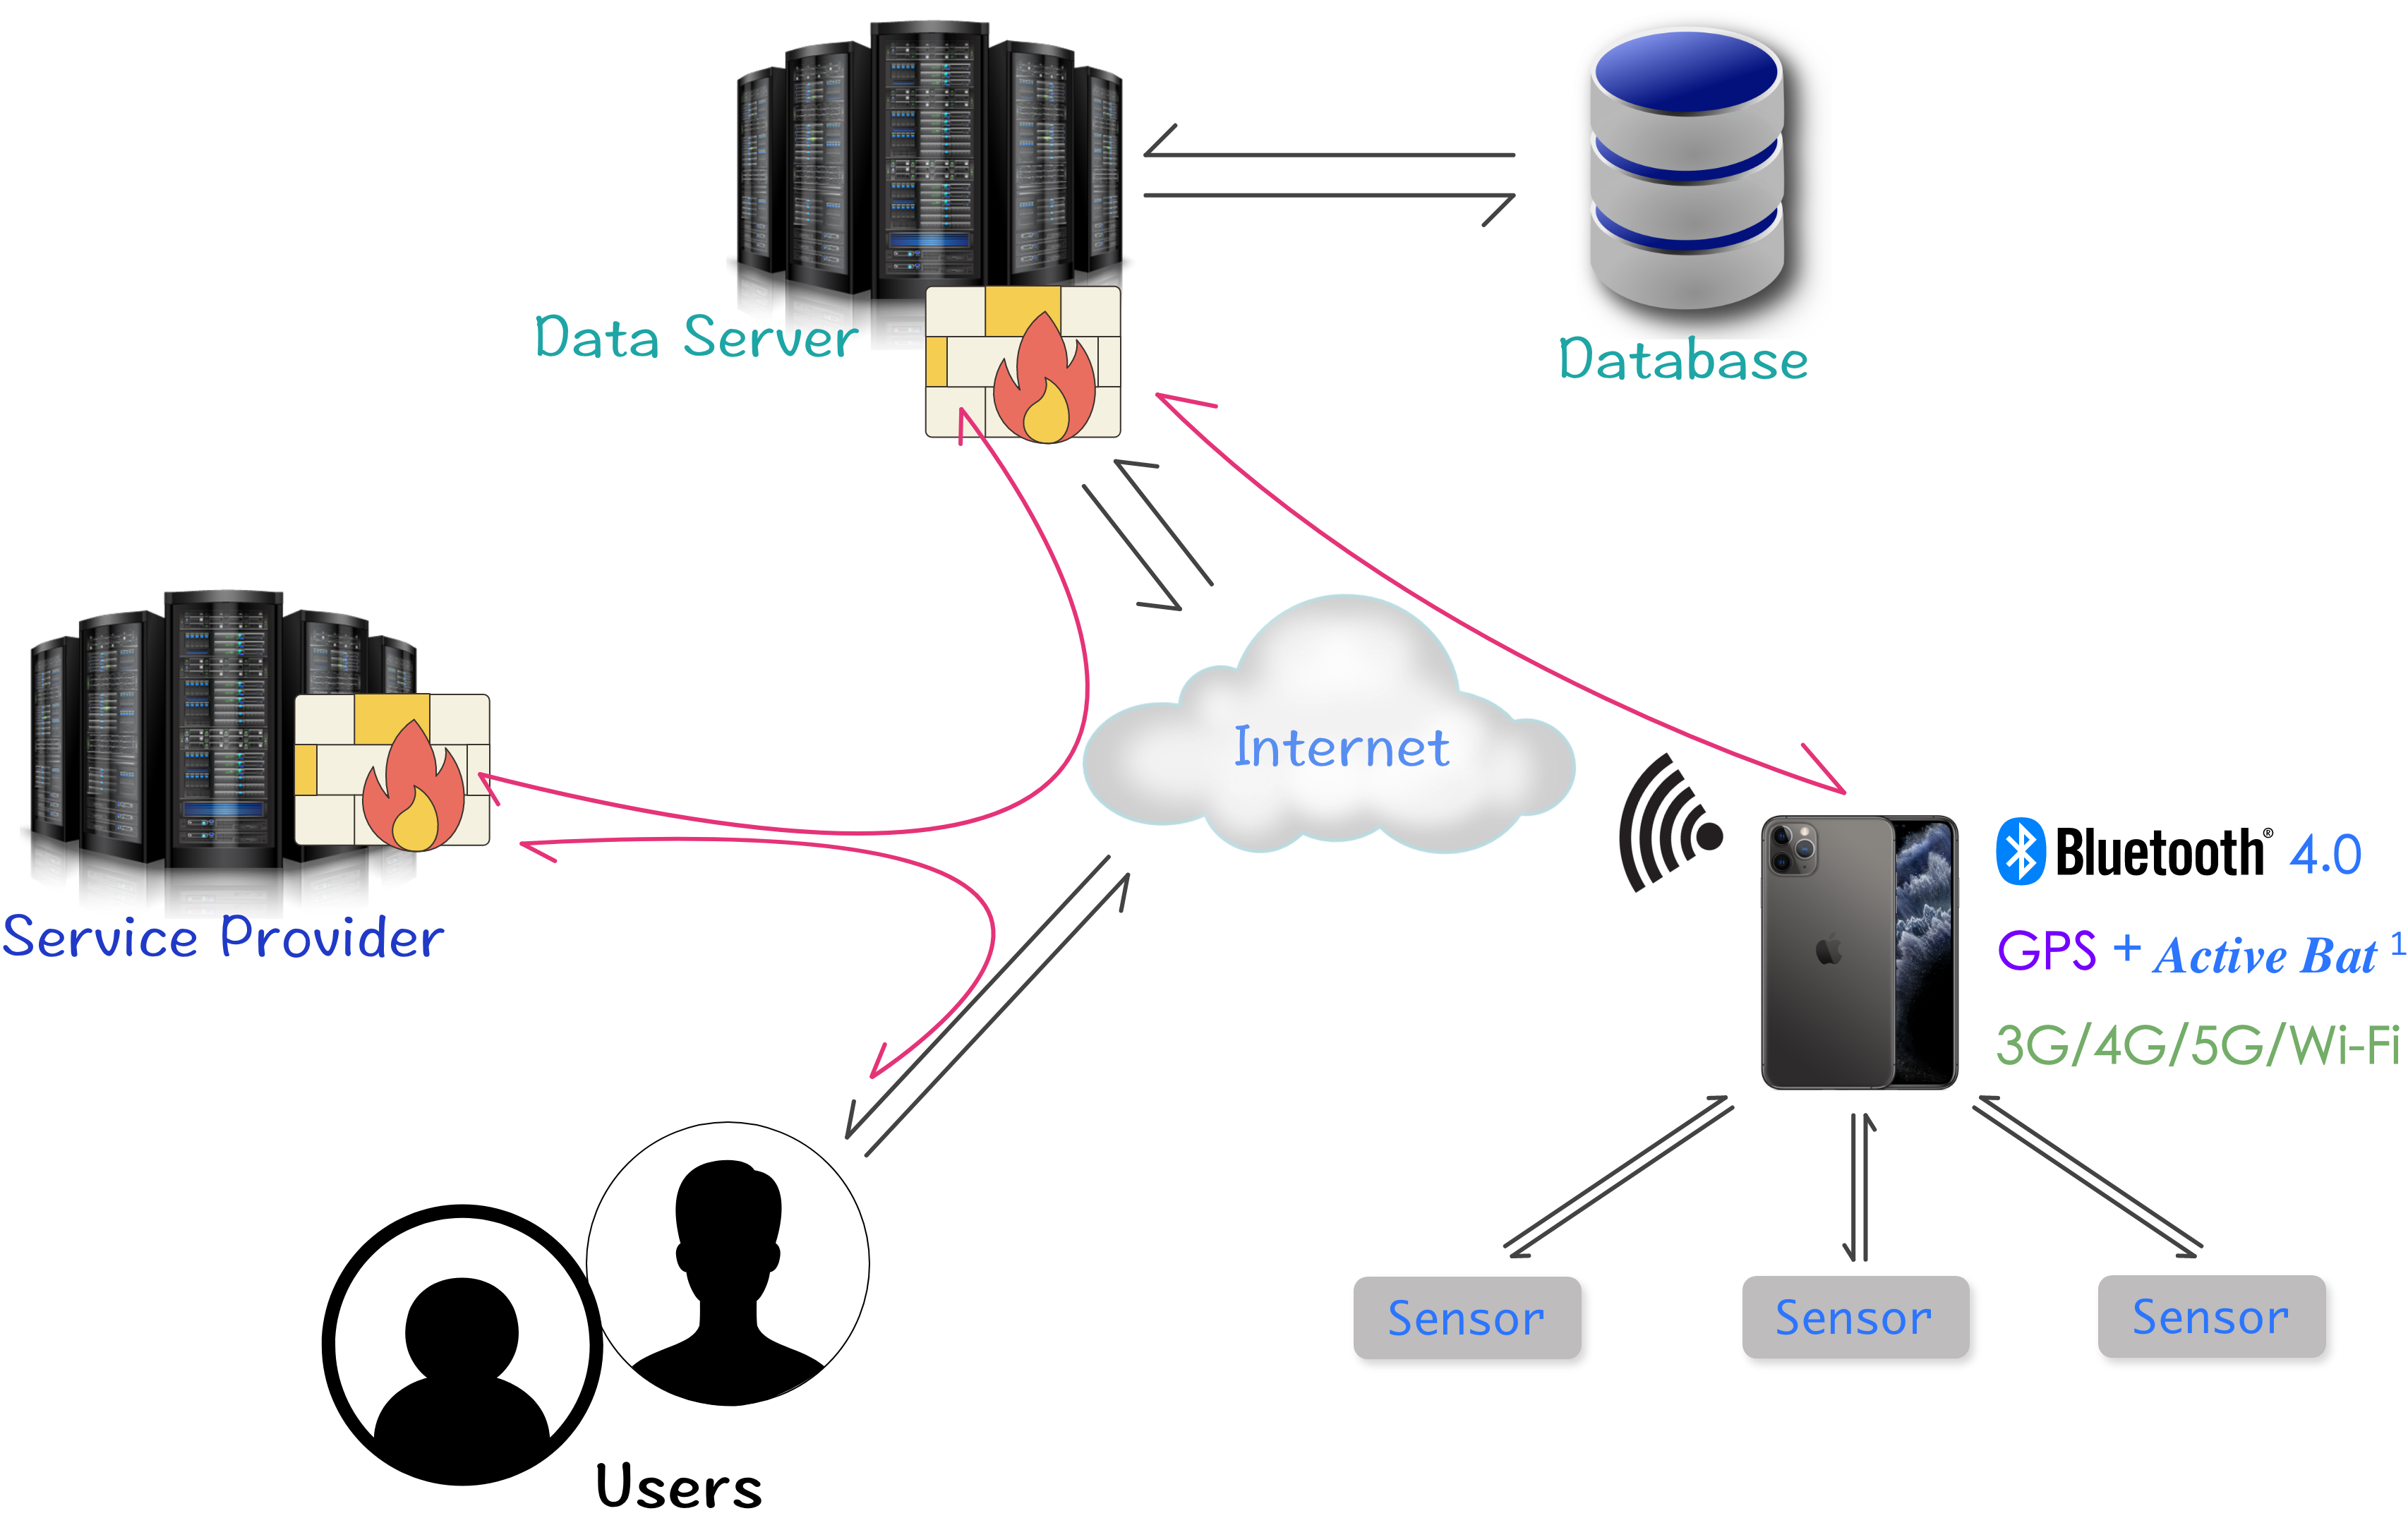
\includegraphics[width=0.5\textwidth]{Architech.png}
%     \caption{Architecture of the IoT System}
%     \label{fig_ar}
% \end{figure}



% Liye Jia

\subsection{Hardware} 
Location systems and various types of sensors are the basis of applications. The location system is mainly used for recording the action routes of confirmed or suspected patients who have an infectious disease, and sensors collect the physical parameters of the human body, such as body temperature, heartbeat, and blood pressure. Moreover, with the consideration of battery life and volume of devices, all of the hardware should be low-powered and miniature. This part contains some details of localization techniques and sensors’ parameters.
\subsubsection{Location System}
The location system can be divided into outdoor and indoor localization. The Global Positioning System (GPS) is a reliable outdoor location system, and it has been generally employed in civilian applications. There are many types of GPS, for instance, Basic GPS (with the lowest accuracy), Real-time Differential GPS (DGPS) with Wide Area Augmentation System (WAAS) (with 2 meters average accuracy), and GPS with Real-time Kinematic (RTK) (with 10 centimeters accuracy)\cite{lamarca2008location}. According to the accuracy required for location, the system, GPS with RTK, is a proper choice. However, GPS with RTK requires massive infrastructures and special units in locating device of clients, so it is really expensive to deploy this system in a region \cite{lamarca2008location}. GPS with WAAS system has cheaper infrastructure and basic devices, and its accuracy usually maintains in 1.8 meters\cite{youssef2003wlan}, which is enough to detect people who have been close to patients of infections and have a high possibility to be infected with the disease. For indoor situations, Wi-Fi devices have been employed by every building as the gateway of the internet, and RADAR estimates the location through the IEEE 802.11 signal strength\cite{lamarca2008location}. Additional infrastructures are not demanded, because its algorithm is based on the database of strength readings of the Wi-Fi signal in the building. Radio scan of Wi-Fi devices can be used in system to estimate the client’s location. When implementing a verification experiment in a 1000 square meters office, the average error is 3 meters if the database is large enough\cite{bahl2000radar}. The accuracy meets the requirements to detect in an apartment which room the user is in. In brief, smartphones can meet every basic condition of GPS and RADAR, so location systems can be easily accomplished through the providers of locating service of smartphones.
\subsubsection{Sensors}
Sensors 




% Yifan Yang
\subsection{Networking}

There are multiple options for creating an IoT network: Wi-Fi, Bluetooth, and ZigBee. 
Each of them has its own characteristics. However, in our system, one specific networking 
technology should be chosen to connect the sensors on people's body and the smart device that has 
internet connection via either Wi-Fi or Cellular. After rough selections and comparison, we narrowed down our candidates to:

\begin{itemize}
    \item Wi-Fi
    \item Bluetooth Classic
    \item ZigBee
    \item Bluetooth Low Energy(BLE)
\end{itemize}

\subsubsection{Wi-Fi}
Wi-Fi is a wireless local area network(WLAN) based on the IEEE 802.11 family of standards that provides internet access within a limited range.
Wi-Fi works in a star topology that has an access point at the center and many devices connected to the access point.
Wi-Fi most commonly uses the 2.4 GHz Ultra High Frequency and 5 GHz Super High Frequency ISM(Industrial, Scientific and Medical) radio bands and has a bandwidth up to 2 MHz which is perfect for data transfer that needs low delay and high data rate. 
However, the high data rate comes with a price. The power consumption is also as high as its data rate. Usually a Wi-Fi device's battery could not last long, for hours or days depending on the battery capacity. 
The range of Wi-Fi could reach tens of meters. However, to ensure a stable connection and stable data transfer, the signal needs to be strong and therefore the device should be relatively close to the access point.

Wi-Fi is currently used as an important technology for WLAN, in industries, homes, and also open areas. It provides a relatively fast and power efficient way for smart devices and computers to get internet access(relative to cellular networks that drains large amount of power). 

\subsubsection{Bluetooth Classic}
Bluetooth operates in the 2.4GHz to 2.485GHz range within the ISM band. Packets are exchanged through one of 79 designated Bluetooth channels each of which has only 1 MHz bandwidth. IEEE used to standardized it as IEEE 802.15.1 but it is no longer maintained. Now, Bluetooth is managed by the Bluetooth Special Interest Group(SIG). Different from Wi-Fi, which is designed as a replacement for high speed cabling for general LAN access, Bluetooth was intended for portable equipment and its applications. Bluetooth is used for creating wireless Personal Area Networks(WPAN). 
Smart Bluetooth devices today like cellphones and laptops are usually equipped with Bluetooth version higher than 4.0, in which Bluetooth Low Energy is integrated with Bluetooth Classic, which means smart devices with Bluetooth 4.0 can connect with devices that use either Bluetooth Classic or Bluetooth Low Energy. 

In the latest Bluetooth version so far, which is Bluetooth 5.2, published on January 6th, 2020, SIG optimized its power consumption performances and support data rates from 1 Mb/s to 3 Mb/s\cite{bluetoothspec2020}. It operates in a Point-to-Point(P2P)(including piconet) network topology\cite{sigwebsite}.

\subsubsection{ZigBee}
ZigBee is a specification for creating Personal Area Networks with small, low-power digital radios. It is based on IEEE 802.15.4 international standard.
It operates in low power and therefore has low data rates. Mostly, ZigBee runs on a mesh topology network, but it can also run on star topology or cluster tree topology based on the requirements. ZigBee uses the 2.4GHz ISM frequency band. It can provide data rate up to 250 kb/s\cite{safaric2006zigbee}. The range of a ZigBee network could reach over 300 meters, and maintains a low power consumption and an low latency. In addition, ZigBee connector devices are relatively small in compare to that of Wi-Fi. ZigBee uses a 64 bit IEEE address or 16 bit NWK(network layer) address for its Media Access Control.

\subsubsection{Bluetooth Low Energy}
Bluetooth Low Energy came out in 2011 as Bluetooth 4.0 and is designed for applications that only needs to exchange small amount of data periodically. The key feature of BLE is its power consumption. It works in a different way from Bluetooth Classic. BLE remains in sleep mode except for when a connection is initiated. Its Physical layer has a data rate of 1 Mb/s. Benefited from the high data rate, a connection time would be established in 3 ms at best, while Bluetooth Classic may take about 100ms. However, the range of Bluetooth Low Energy is a little bit shorter than that of ZigBee. 

BLE operates in the same frequency band as Bluetooth Classic, which is 2.4 GHz ISM band(2.402-2.480 GHz Utilized)\cite{sigwebsite}. It divides the frequency range into 40 channels with 2 MHz spacing, 3 of which are advertising channels for establishing connections and 37 of which are data channels.
In the latest Bluetooth version so far, which is Bluetooth 5.2, published on January 6th, 2020, Bluetooth Low Energy supports multiple Physical Layer options that support data rates from 125 kb/s to 2 Mb/s, multiple power levels from 1 mW to 100 mW\cite{sigwebsite, gomez2012overview}. 
BLE uses a 32 bit address for Media Access Control, which means the theoretical number of connections is $ 2^{32} $. BLE could run on Point-to-Point, Broadcast, and Mesh topology, Making the structure of the network more flexible.

Also, in the latest version(5.2), a new feature of Bluetooth Low Energy Power Control, also known as LE Power Control(LEPC), is introduced. Power control for wireless communication is controlling the power level of a transmitter to achieve better communication signals or quality of service, including the optimization of power consumption\cite{bluetoothspec2020}. LE Power Control works in a way that when two Bluetooth devices establish a connection, at a certain moment, one device is in a transmitting state, and the peer device is in a receiving state. Usually, the receiver requires a certain signal-to-noise ratio (SNR), and the power level of the transmitter shouldn't be too high or too low. 

\begin{itemize}
    \item If the power level of the transmitter is too high, it may cause the receiver device to be saturated and result in link failure. And it wastes power on the transmitter side.
    \item If the power level of the transmitter is too low, the receiver can receive the packets from the transmitter, but the packet error rate (PER) can become high.
\end{itemize}

The LE Power Control feature can be used to adjust a connected peer device’s transmit power level based on the receiver’s signal level.\cite{bluetoothspec2020}
This further optimized the power consumption of Bluetooth, made the link quality better, and minimized interference and noise over the air against nearby devices. 


\subsubsection*{System Requirements Analysis}
In our IoT system, we are choosing a network technology for the connection between body sensors and the local smart device, which is the cellphone in this situation. Our sensors need to be as small as possible and the power supply is limited while the battery life needs to be relatively long. Users don't want to change battery or charge all the sensors every day or every a few days. Therefore, the power consumption is an important part when considering a network. Based on the application, our sensors are connected to the phone, which is not far from the person himself. The network could thus work in a short distance. In Table \ref{table_spec}, we can see the specifications for these networks. Sensors works in different schedules and report its data periodically that is controlled by the smart device. The amount of data transferred is limited and the speed of connection does not need to be high. For the purpose of reduce power consumption to gain longer battery life and a smaller battery, Wi-Fi and Bluetooth Classic is not considered suitable for this application. 

\begin{table}[!t]
\renewcommand{\arraystretch}{1.3}
\caption{Technical Specification of Various Networks}
\label{table_spec}
\centering
\resizebox{0.5\textwidth}{!}{%
\begin{tabular}{@{}lcccc@{}}
\toprule
Technical Specification & Wi-Fi & Bluetooth Classic & ZigBee & BLE \\ \midrule
Distance/Range          & $\geq300m$  & $100m$ &    $300m$    & $\geq100m$ \\
Data Rate  &   54 Mb/s    & 1-3 Mb/s &  250 kb/s  &  0.25-2 Mb/s     \\
Battery Life  & hours/days & days/months &   months/years &  months/years   \\ \bottomrule
\end{tabular}
}
\end{table}

Between ZigBee and Bluetooth Low Energy, there are some similarities but also some differences. They both have the ability to sleep in order to save energy. However, the power consumption performances are still different.  
Based on previous studies\cite{siekkinen2012low}, BLE indeed consumes extremely little energy and has a very attractive ratio of energy per bit transmitted. After further technology developments over the years, Adaptive Frequency Hopping(AFH) is implemented and integrated into BLE, combating the interference and improving the connection quality. BLE is now a desirable option for our system. With a extremely low energy consumption, a low data rate that can sufficiently support the data exchange, and a distance that is much further than needed, a BLE device could run years without changing batteries. However, that is almost the time to get a new device. In addition, the ecosystem of Bluetooth is far better than that of ZigBee. Bluetooth devices running mobile operating systems including Android, iOS, Windows Phone, and BlackBerry, as well as macOS, Linux, Windows 8 and Windows 10 natively support Bluetooth Low Energy, which ZigBee could not achieve. Therefore, Bluetooth Low Energy is the choice for our IoT system.

\subsubsection*{Network Topology and Structure}

In most cases, we assume that the smartphone is with the person. Therefore, sensors could connect to the smartphone in a Point-to-Point star topology as shown in Fig \ref{fig_topology}. 
The smartphone, as a center master, could send command or data by broadcasting to all devices or could send a specific command to a certain device that controls its frequency of reporting data or to bind device with the smartphone and negotiate their tokens for encryption and identification. 

\begin{figure}[!t]
    \centering
    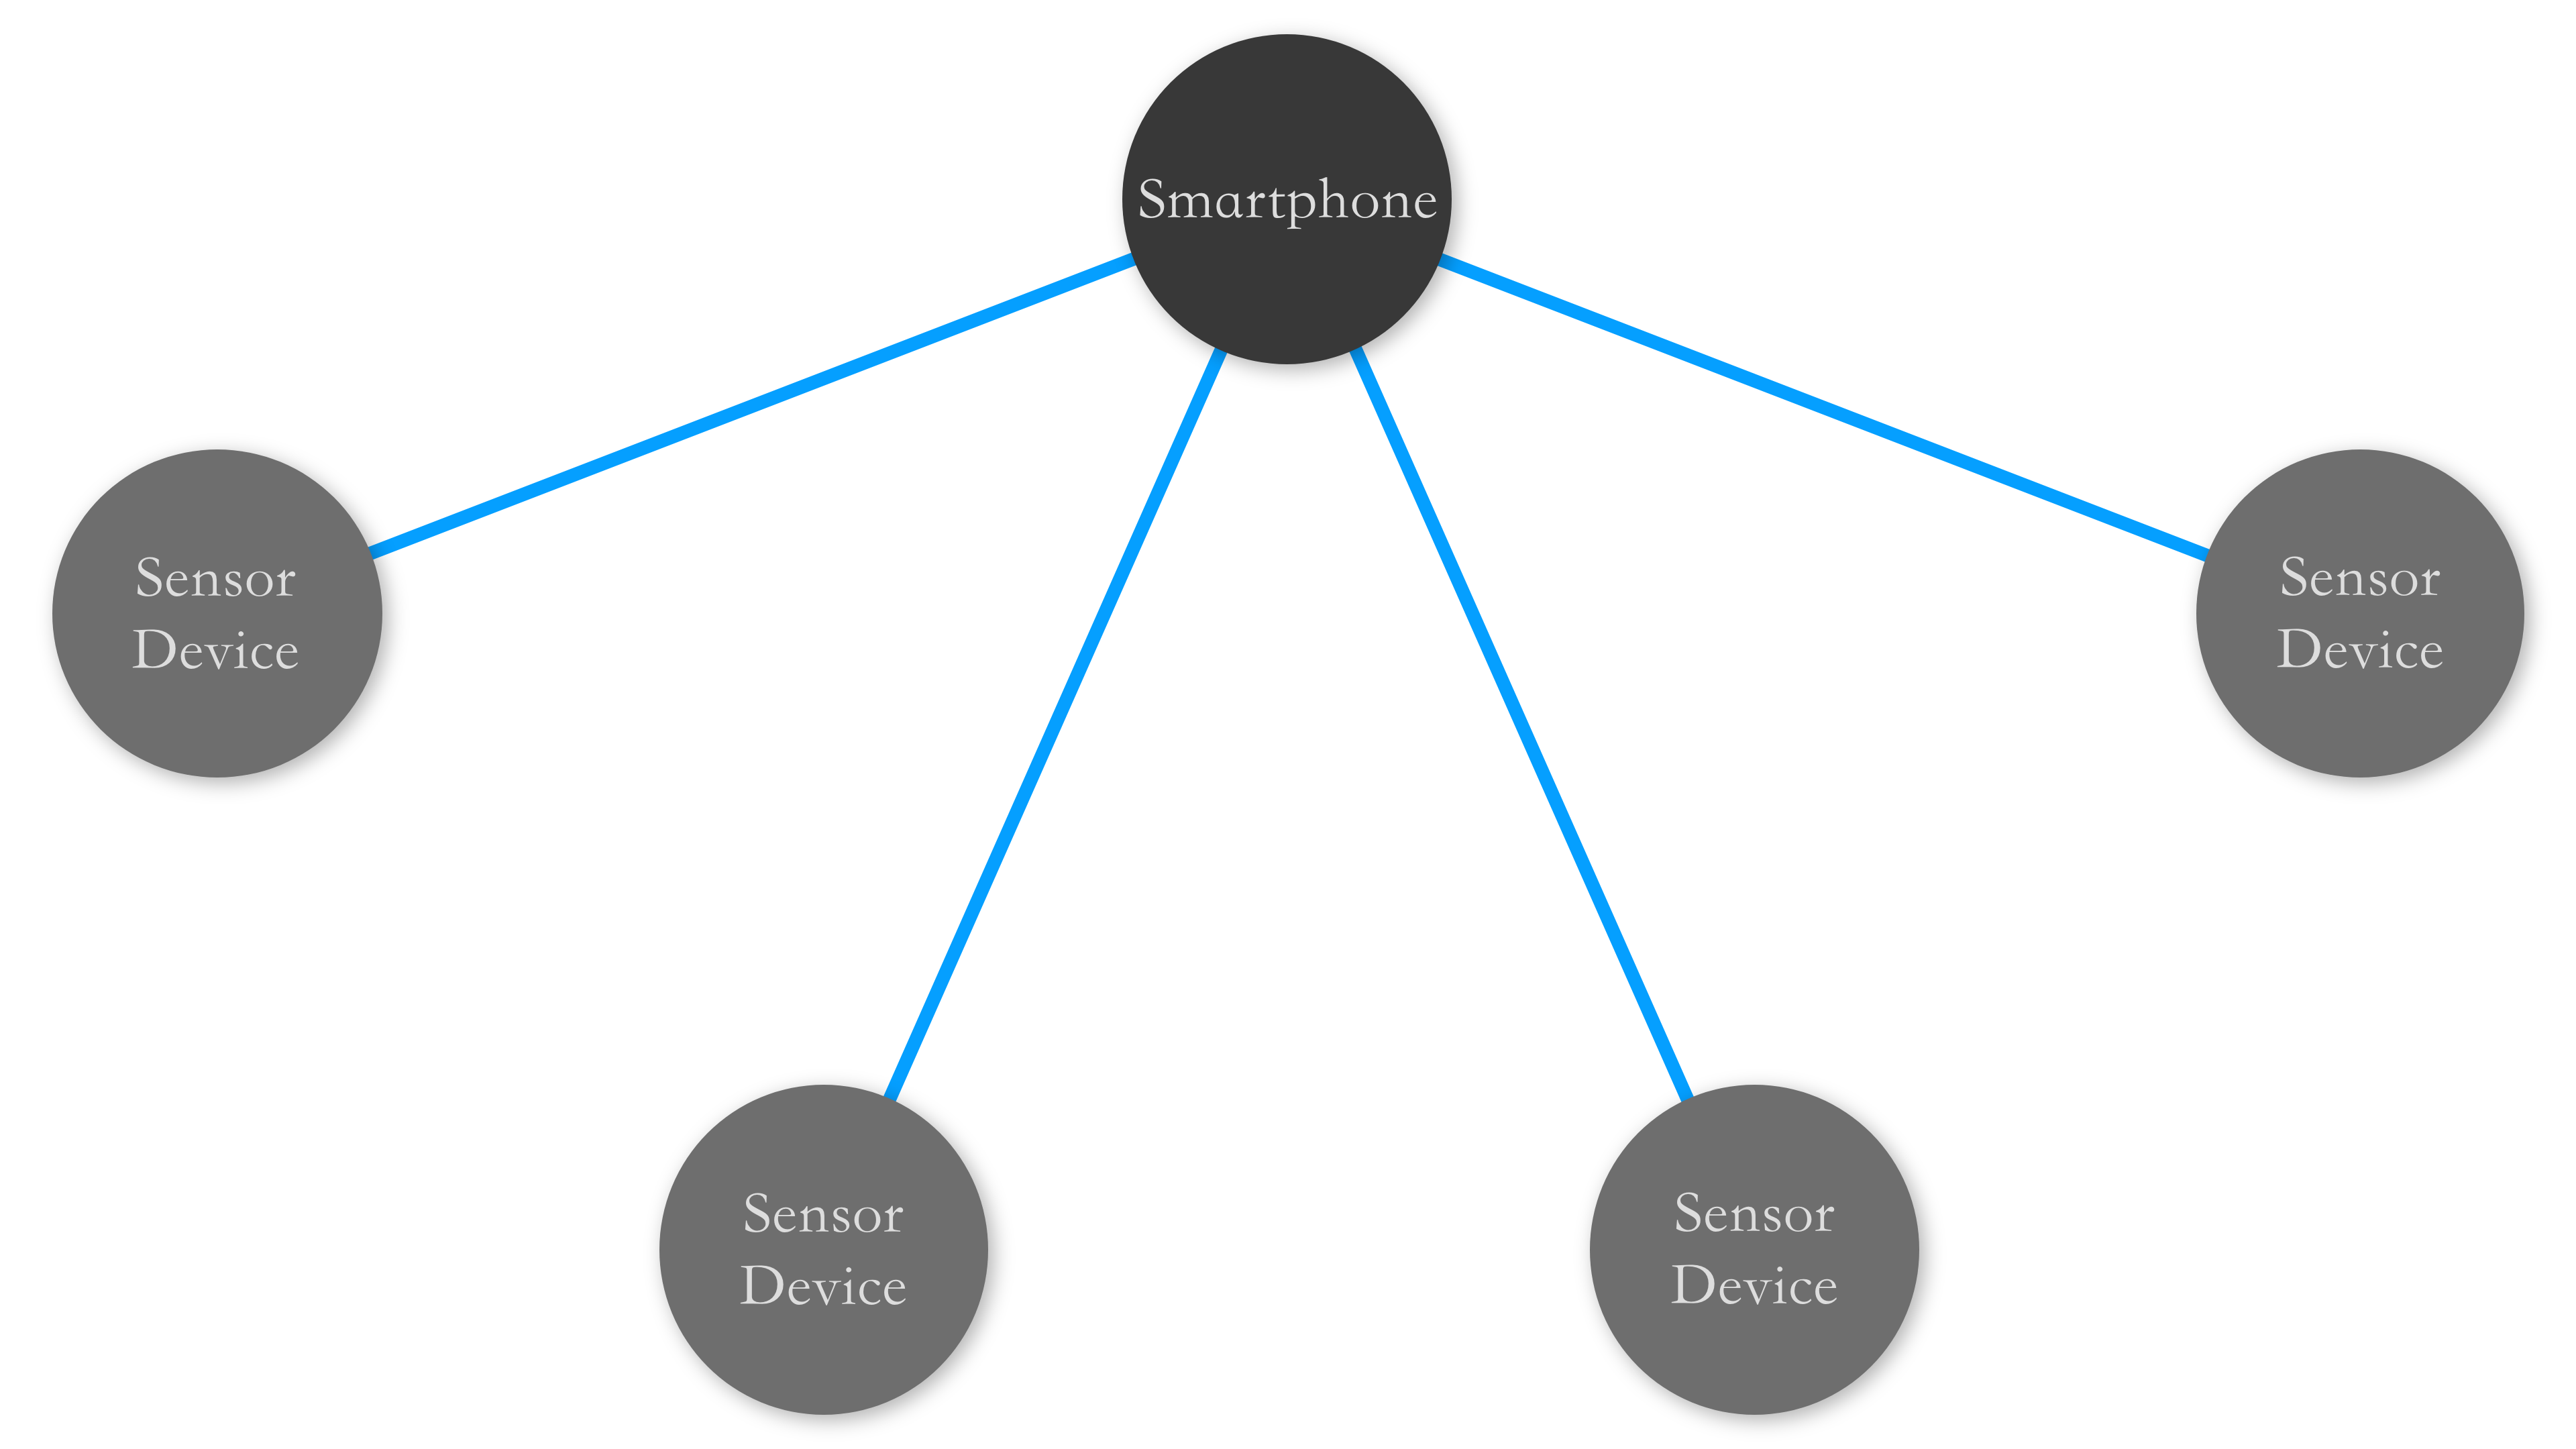
\includegraphics[width=0.5\textwidth]{Topology-Labeled.png}
    \caption{BLE Star Topology}
    \label{fig_topology}
\end{figure}



% Yujie Wang
\subsection{Internet Data Flow}


Your section goes here, Wang.






% Yangkai Lin
\subsection{Application Layer}

Kai, this is your section, right?\cite{springer.978.3.030.34986.8.Chapter.720200101}

\subsubsection{Cloud Computing and Database}



\subsubsection{Other Concerns}






\section{Use Case Scenarios}
Paragraph one Paragraph one Paragraph one Paragraph one Paragraph one 
Paragraph one Paragraph one Paragraph one Paragraph one Paragraph one 
Paragraph one Paragraph one Paragraph one Paragraph one Paragraph one 
Paragraph one Paragraph one Paragraph one Paragraph one Paragraph one 
Paragraph one Paragraph one Paragraph one Paragraph one Paragraph one 

Paragraph two Paragraph two Paragraph two Paragraph two Paragraph two 
Paragraph two Paragraph two Paragraph two Paragraph two Paragraph two 
Paragraph two Paragraph two Paragraph two Paragraph two Paragraph two 
Paragraph two Paragraph two Paragraph two Paragraph two Paragraph two 
Paragraph two Paragraph two Paragraph two Paragraph two Paragraph two 

\section{Conclusion}

Paragraph one Paragraph one Paragraph one Paragraph one Paragraph one 
Paragraph one Paragraph one Paragraph one Paragraph one Paragraph one 
Paragraph one Paragraph one Paragraph one Paragraph one Paragraph one 
Paragraph one Paragraph one Paragraph one Paragraph one Paragraph one 
Paragraph one Paragraph one Paragraph one Paragraph one Paragraph one 

Paragraph two Paragraph two Paragraph two Paragraph two Paragraph two 
Paragraph two Paragraph two Paragraph two Paragraph two Paragraph two 
Paragraph two Paragraph two Paragraph two Paragraph two Paragraph two 
Paragraph two Paragraph two Paragraph two Paragraph two Paragraph two 
Paragraph two Paragraph two Paragraph two Paragraph two Paragraph two 

\section*{Acknowledgments}

Paragraph one Paragraph one Paragraph one Paragraph one Paragraph one 
Paragraph one Paragraph one Paragraph one Paragraph one Paragraph one 
Paragraph one Paragraph one Paragraph one Paragraph one Paragraph one 
Paragraph one Paragraph one Paragraph one Paragraph one Paragraph one 
Paragraph one Paragraph one Paragraph one Paragraph one Paragraph one 

Paragraph three

\bibliographystyle{IEEEtran}
\bibliography{References}
\end{document}